%%%%%%%%%%%%%%%%%%%%%%%%%%%%%%%%%%%%%%%%%
% Beamer Presentation
% LaTeX Template
% Version 1.0 (10/11/12)
%
% This template has been downloaded from:
% http://www.LaTeXTemplates.com
%
% License:
% CC BY-NC-SA 3.0 (http://creativecommons.org/licenses/by-nc-sa/3.0/)
%
%%%%%%%%%%%%%%%%%%%%%%%%%%%%%%%%%%%%%%%%%

%----------------------------------------------------------------------------------------
%    PACKAGES AND THEMES
%----------------------------------------------------------------------------------------

\documentclass{beamer}

\usepackage[utf8]{inputenc}
\usepackage[T1]{fontenc}
\usepackage{graphicx}
\usepackage{listings}

\mode<presentation> {

% The Beamer class comes with a number of default slide themes
% which change the colors and layouts of slides. Below this is a list
% of all the themes, uncomment each in turn to see what they look like.

%\usetheme{default}
%\usetheme{AnnArbor}
%\usetheme{Antibes}
%\usetheme{Bergen}
%\usetheme{Berkeley}
%\usetheme{Berlin}
%\usetheme{Boadilla}
%\usetheme{CambridgeUS}
%\usetheme{Copenhagen}
%\usetheme{Darmstadt}
%\usetheme{Dresden}
%\usetheme{Frankfurt}
%\usetheme{Goettingen}
%\usetheme{Hannover}
%\usetheme{Ilmenau}
%\usetheme{JuanLesPins}
%\usetheme{Luebeck}
\usetheme{Madrid}
%\usetheme{Malmoe}
%\usetheme{Marburg}
%\usetheme{Montpellier}
%\usetheme{PaloAlto}
%\usetheme{Pittsburgh}
%\usetheme{Rochester}
%\usetheme{Singapore}
%\usetheme{Szeged}
%\usetheme{Warsaw}

% As well as themes, the Beamer class has a number of color themes
% for any slide theme. Uncomment each of these in turn to see how it
% changes the colors of your current slide theme.

%\usecolortheme{albatross}
%\usecolortheme{beaver}
%\usecolortheme{beetle}
%\usecolortheme{crane}
%\usecolortheme{dolphin}
%\usecolortheme{dove}
%\usecolortheme{fly}
%\usecolortheme{lily}
%\usecolortheme{orchid}
%\usecolortheme{rose}
%\usecolortheme{seagull}
\usecolortheme{seahorse}
%\usecolortheme{whale}
%\usecolortheme{wolverine}

%\setbeamertemplate{footline} % To remove the footer line in all slides uncomment this line
%\setbeamertemplate{footline}[page number] % To replace the footer line in all slides with a simple slide count uncomment this line

%\setbeamertemplate{navigation symbols}{} % To remove the navigation symbols from the bottom of all slides uncomment this line
}

\usepackage{graphicx} % Allows including images
\usepackage{booktabs} % Allows the use of \toprule, \midrule and \bottomrule in tables

%----------------------------------------------------------------------------------------
%    TITLE PAGE
%----------------------------------------------------------------------------------------

\title[Linux Container APIs]{Container management APIs} % The short title appears at the bottom of every slide, the full title is only on the title page

\author{Serge Hallyn} % Your name
\institute[Canonical] % Your institution as it will appear on the bottom of every slide, may be shorthand to save space
{
Canonical, Ltd \\ % Your institution for the title page
\medskip
\textit{serge.hallyn@ubuntu.com} % Your email address
}
\date{\today} % Date, can be changed to a custom date

\begin{document}

\lstset{language=sh}

\begin{frame}
\titlepage % Print the title page as the first slide
\end{frame}

\begin{frame}
\begin{figure}
  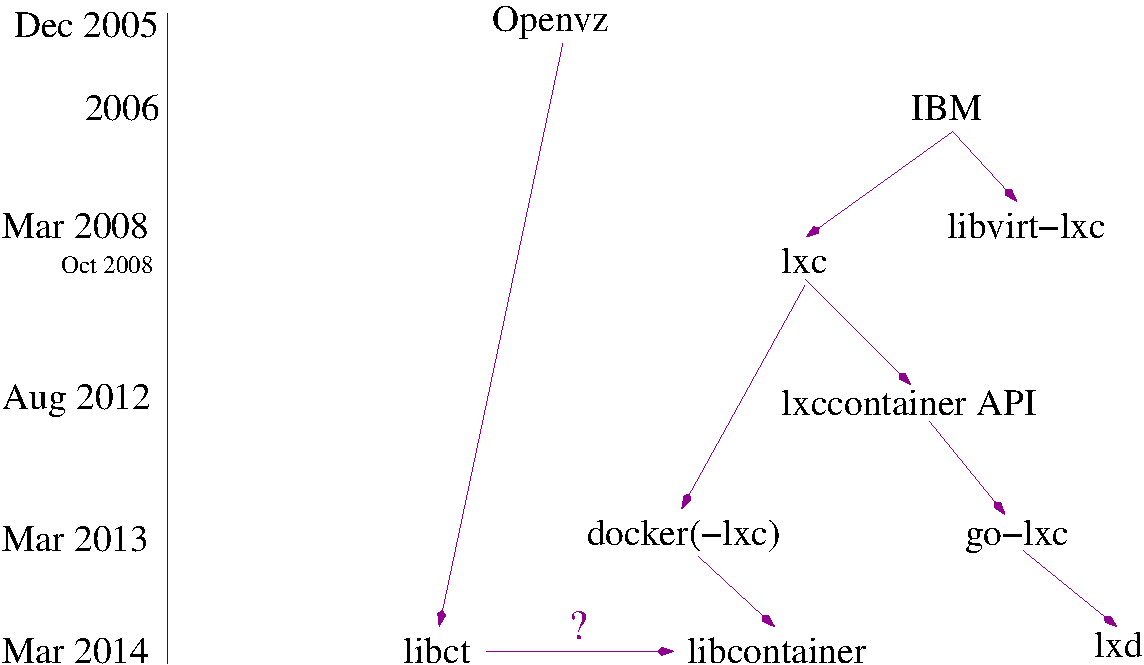
\includegraphics[width=\textwidth]{timeline.pdf}
\end{figure}
\end{frame}

\begin{frame}
\frametitle{Regular Usage: Overview}
\begin{itemize}
\item Let's first go over the basics:
  \begin{itemize}
  \item Download an image
  \item Run a command in a container
  \item Publish the new image
  \end{itemize}
\end{itemize}
\end{frame}

\begin{frame}[fragile]
\frametitle{Regular Usage: Docker}
\begin{itemize}
\item docker pull ubuntu
\item docker run -i -t ubuntu /usr/bin/touch cd
\item docker ps -a
{\tiny
\begin{verbatim}
ef45ea2cf7da        ubuntu:latest       "/usr/bin/touch cd"   10 seconds ago
d7bd5a48055f        ubuntu:latest       "/bin/bash"           19 hours ago
\end{verbatim}
}

\item docker run -i -it ubuntu /bin/ls
\item docker commit -m "add ab" f57b28609407 ubuntu:ab
{\tiny
\verb@f68322852844620ea3a0ee9fc86ae7f2016f344d031e80a5331fffaa8efcf61c@
}

\item sudo docker images
{\tiny
\begin{verbatim}
REPOSITORY          TAG                 IMAGE ID            CREATED             VIRTUAL SIZE
ubuntu              cd                  f68322852844        21 seconds ago      188.3 MB
ubuntu              latest              91e54dfb1179        4 weeks ago         188.3 MB
\end{verbatim}
}
\end{itemize}
\end{frame}

\begin{frame}
\frametitle{Regular Usage: LXD}
\begin{itemize}
\item lxc image list lxc:
\item lxc launch lxc:ubuntu/trusty/amd64 u1
\item lxc image list
\item lxc list
\item lxc exec u1 -- /usr/bin/touch/cd
\item lxc stop u1
\item lxc publish u1 myrepo:ubuntucd
\end{itemize}
\end{frame}

\begin{frame}
\frametitle{Regular Usage: LXC}
\begin{itemize}
\item lxc-create -B btrfs -t download -n u1 -- -d ubuntu -r trusty -a amd64
\item lxc-ls -f
\item lxc-start -n u1
\item lxc-attach -n u1 -- touch /cd
\item lxc-stop -n u1
\item lxc-clone -s -o u1 -n u2
\item \texttt{Not image-based - no `publish' concept}
\end{itemize}
\end{frame}

\begin{frame}
\frametitle{Digging Deeper}
\begin{itemize}
\item Getting familiar with the commands is important
\item Docker and LXD have REST APIs
\item Go further building custom tools against library APIs
\end{itemize}
\end{frame}

\begin{frame}[fragile]
\frametitle{Docker REST API}
\begin{itemize}
\item List Images: \\
curl --unix-socket /run/docker.sock http:/images/json
\item Create a container: \\
\begin{lstlisting}
curl --unix-socket /run/docker.sock \
  -H "Content-Type: application/json" \
  -X POST http:/containers/create \
  -d '{ "Image": "ubuntu:latest", \
  "ExposedPorts":{"22/tcp":{}} , \
  "Binds": ["/home/ubuntu:/opt"], \
  "Entrypoint": "/sbin/init"}' \\
\end{lstlisting}
  \vspace{0.25in}
\textbf{ {"Id":"3b7e4b7aa...","Warnings":null} } \\

\item Start the container: \\
curl --unix-socket /run/docker.sock \
  -X POST http:/containers/ID/start \
  -d '{ "Binds":["/home/serge:/opt"] }'
\end{itemize}
\end{frame}

\begin{frame}
\begin{itemize}
\item curl --unix-socket /run/docker.sock -X GET http:/containers/json
\item curl --unix-socket /run/docker.sock -X POST http:/containers/ID/stop
\item curl --unix-socket /run/docker.sock -X DELETE  http:/containers/ID
\item curl --unix-socket /run/docker.sock -X DELETE  http:/containers/log
\item curl --unix-socket /run/docker.sock -X GET http:/containers/ID/logs?stdout=1
\end{itemize}
\end{frame}

\begin{frame}
\frametitle{Runc}
\begin{itemize}
\item A new way to run OpenContainers format containers
\item Requires
  \begin{itemize}
  \item untarred rootfs
  \item config.json: mounts (brief), user, env, capabilities, arch
  \item runtime.json: mounts(details), devices, security, hooks, more
  \end{itemize}
\end{itemize}
\end{frame}

\begin{frame}[fragile]
\frametitle{LXD REST API}
\begin{itemize}
\item List images: \\
{\tiny
  \begin{lstlisting}
curl --unix-socket /var/lib/lxd/unix.socket http:/1.0
  \end{lstlisting}
}

%\end{itemize}
%\end{frame}
%
%\begin{frame}[fragile]
%\begin{itemize}
%\item Create container: \\
%{\tiny
%  \begin{lstlisting}
%curl --unix-socket /var/lib/lxd/unix.socket http:/1.0/containers \
%  -X POST -d '{  "name":"x1", "source":{"type":"image","alias":"ubuntu" } }'
%  \end{lstlisting}
%}
%
%{\tiny
%\begin[verbatim}
%{"type":"async","status":"OK",
%"status_code":100,
%"operation":"/1.0/operations/e8b807a6-e19a-4cfe-ad69-2069ecaec14a",
%"resources":{"containers":["/1.0/containers/x1"]},
%"metadata":null}
%\end{verbatim}
%}

\item All documented at: \\
{\tiny
\url{https://github.com/lxc/lxd/blob/master/specs/rest-api.md}
}
\end{itemize}
\end{frame}

\begin{frame}[fragile]
\frametitle{Building new tools: lxd/lxc}
{\bf Create container in go:} \\
{\tiny
\begin{lstlisting}
func create(name, lxcpath string) error {
  c, err := lxc.NewContainer(name, lxcpath)
  if err != nil {
    return err
  }
  options := lxc.TemplateOptions{
    Template:             "download",
    Distro:               "ubuntu",
    Release:              "trusty",
    Arch:                 "amd64",
    FlushCache:           false,
    DisableGPGValidation: false,
  }
  err = c.Create(options)
  return err
\end{lstlisting}
}
\end{frame}

\begin{frame}[fragile]
\frametitle{Building new tools: lxd/lxc}
{\bf Get state of running container in python:} \\
{\tiny
\begin{lstlisting}
>>> import lxc
>>> c=lxc.Container("x1", "/var/run/lxd/containers")
>>> c.state
"RUNNING"
\end{lstlisting}
}
\end{frame}

\begin{frame}
\frametitle{Building new tools: libct}
\begin{itemize}
\item Libct is focused on creating container drivers
\item No concept of configuration files or image formats
\item Intended to be flexible
  \begin{itemize}
  \item Any combination of namespace sharing
  \item Any combination of security features
  \item Mount as you wish
  \item \dots you must do it all yourself
  \end{itemize}
\item Assume we create a container with lxc-start or docker,
\item Run "ps" in the container
\end{itemize}
\end{frame}

\begin{frame}[fragile]
\frametitle{Building new tools: libct}
{\bf Run container:} \\
{\tiny
\begin{lstlisting}
...
\end{lstlisting}
}
\end{frame}

\begin{frame}
\frametitle{Building new tools: libcontainer}
\begin{itemize}
\item Written in go \\
only usable in go
\item To use outside of go: {\em runc}
\end{itemize}

\end{frame}


%------------------------------------------------

\end{document} 
